\documentclass[DM,toc]{lsstdoc}
\usepackage{booktabs}

\title[Qserv Test 2013]{Qserv 300 Node Test}
\author{Jacek~Becla}
\date{2013-10-06}
\setDocRef{DMTR-12}

\setDocAbstract{%
The largest test we run to-date was run during July-September of 2013 on a 300-node cluster at the IN2P3 center in France. The main purpose of the test was to test Qserv scalability and performance beyond 150 nodes, and re-check concurrency at scale.
For comparisons, the previous large scale test can be found in \citeds{DMTR-21}.
}

\begin{document}
\maketitle

\section{Hardware}
Test machines were quad-core Intel(R) Xeon L5430 running at 2.66\,GHz speed, with small local spinning disks (120\,GB of usable space), and 16\,GB of RAM per machine. We received an allocation of 320 nodes, which was intended to allow for a 300 node test in spite of some failed nodes (and indeed, 17 nodes failed during the tests!)

\section{Data}
With only 120\,GB of available storage per node, only a limited amount of data could get produced. We tuned our data synthesizer to produce 50\,GB of table data per node, giving 15\,TB of aggregate data. 220\,GB of LSST PT1.2 data \citedsp{Document-9044} was synthesized into a dense stripe covering the declination range -9deg. to +9deg, setting the partitioning to 120 stripes and 9 substripes (1.5\,deg $\times$ 1.5\,deg chunks and 10\,arc-minute-sided subchunks). This yielded 3,000 chunks of data, with 9 to 11 chunks of data on each node. The Object table had 0.4 billion rows, and the Source table had 14 billion rows. Data partitions for the Source table averaged 4\,GB.

Data synthesis took a couple hours for the Object table and overnight for the Source table. Recent work on the installation software enabled data loading ingest to happen within a couple hours (comparing to $\sim$6 days for the 150-node test we run two years earlier.)

\section{Software stability issues identified}

The initial Qserv installation did not function for queries involving 300 nodes, even though subsets involving 10, 50, 100, and 150 nodes functioned properly. The first culprit was the use of an older XRootD release that was missing recent patches for a particular client race condition. Another culprit was instability exacerbated by excessive use of threads in the original threading model that the testing in section 9.5 was to address. This was addressed by re-tuning relevant threading constants. The new XRootD client we are working on (expected to be ready in November of 2013) is expected to further improve thread management.

\section{Queries}

\subsection{Low volume – object retrieval}

\begin{quote}
\begin{lstlisting}[language=SQL]
SELECT * FROM Object WHERE objectId = <id>
\end{lstlisting}
\end{quote}

End-to-end user execution time averaged at 1.1 seconds.

\subsection{Low volume – small area search}

\begin{quote}
\begin{lstlisting}[language=SQL]
SELECT	count(*)
FROM	Object
WHERE	qserv_areaspec_box(1,3,2,4) AND
	scisql_fluxToAbMag(zFlux_PS) BETWEEN 21 AND 21.5
\end{lstlisting}
\end{quote}

This average query response time was 1.3 sec. This is roughly the minimum end-to-end execution time for query that selects small region for this version of Qserv.

\subsection{Low volume – small area search with additional conditions}

\begin{quote}
\begin{lstlisting}[language=SQL]
SELECT	count(*) FROM Object
WHERE	qserv_areaspec_box(1,2,3,4)
AND	scisql_fluxToAbMag(zFlux_PS) BETWEEN 21 AND 21.5
AND	scisql_fluxToAbMag(gFlux_PS)-
	  scisql_fluxToAbMag(rFlux_PS) BETWEEN 0.3 AND 0.4
AND	scisql_fluxToAbMag(iFlux_PS)-
	  scisql_fluxToAbMag(zFlux_PS) BETWEEN 0.1 AND 0.12
\end{lstlisting}
\end{quote}

This average query response time was 1.3 sec. The extra CPU expense of the conditions was insignificant.

\subsection{Low volume – simple join}

\begin{quote}
\begin{lstlisting}[language=SQL]
SELECT	s.ra, s.decl
FROM	Object o
JOIN	Source s USING (objectId)
WHERE	o.objectId = 142367243760566706
AND	o.latestObsTime = s.taiMidPoint
\end{lstlisting}
\end{quote}

This returned in an average time of 11.2 sec.

\subsection{High volume – object count}

\begin{quote}
\begin{lstlisting}[language=SQL]
SELECT COUNT(*) FROM Object
\end{lstlisting}
\end{quote}

End-to-end user execution time averaged 7.8 seconds. This is the minimum overhead to dispatch queries for all 3,000 chunks to all 300 nodes and retrieve their results. A condition-less \texttt{COUNT(*)} is executed as a metadata lookup by MySQL when using MyISAM tables, involving almost no disk I/O.
Similar query executed on the Source table returned in 11.9 seconds.

\subsection{High volume – full Object scans}

\begin{quote}
\begin{lstlisting}[language=SQL]
SELECT COUNT(*) FROM LSST.Object WHERE gFlux_PS>1e-25
\end{lstlisting}
\end{quote}

This query was repeated with different constants in the filtering condition, and the execution time did not vary significantly – it returned in an average time of 8.45 sec – or less than 1 second longer than the condition-less
\texttt{COUNT(*)} query.

\begin{quote}
\begin{lstlisting}[language=SQL]
SELECT	objectId, ra_PS, decl_PS, uFlux_PS, gFlux_PS,
	rFlux_PS,iFlux_PS, zFlux_PS, yFlux_PS
FROM	Object
WHERE	scisql_fluxToAbMag(iFlux_PS)-
	scisql_fluxToAbMag(zFlux_PS)>4
\end{lstlisting}
\end{quote}

Varying the flux difference filter in a range of 4-5, the execution time ranged between 7-9 seconds.

\begin{quote}
\begin{lstlisting}[language=SQL]
SELECT	objectId, ra_PS, decl_PS,
	scisql_fluxToAbMag(zFlux_PS)
FROM	LSST.Object
WHERE	scisql_fluxToAbMag(zFlux_PS) BETWEEN 25 AND 26
\end{lstlisting}
\end{quote}

End-to-end execution time ranged from 7.7 to 8.4 seconds.

\subsection{High volume – Source table scan}

\begin{quote}
\begin{lstlisting}[language=SQL]
SELECT	objectId
FROM	Source
JOIN	Object USING(objectId)
WHERE	qserv_areaspec_box(1,3,2,4)
\end{lstlisting}
\end{quote}

This returned in 9 min 42.9 sec. Some portion of this time was spent printing the results to the screen (this test utilized a standard MySQL command-line client).
9.5.3.8 Super-high volume – near neighbor

\begin{quote}
\begin{lstlisting}[language=SQL]
SELECT	COUNT(*) FROM Object o1, Object o2
WHERE	qserv_areaspec_box(-5,-5,5,5)
AND	scisql_angSep(o1.ra_PS, o1.decl_PS,
		o2.ra_PS, o2.decl_PS) < 0.1
\end{lstlisting}
\end{quote}

This query finds pairs of objects within a specified spherical distance which lie within a large part of the sky (100 deg$^2$ area). The execution times was 4 min 50 sec. The resultant row counts was $\sim$7 billion.
\section{Scaling}

We run a subset of the above queries on different number nodes (50, 100, 250, 200, 250, 300), in ``week scaling'' configuration, to determine how our software scales.

\begin{figure}
	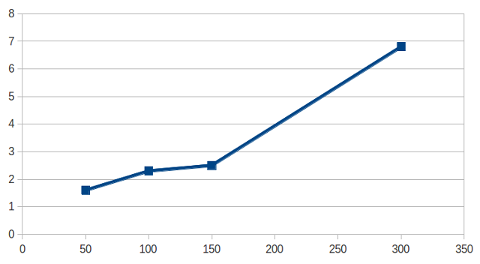
\includegraphics[width=\textwidth]{f1}
	\caption{}
	\label{fig:1}
\end{figure}

\begin{figure}
	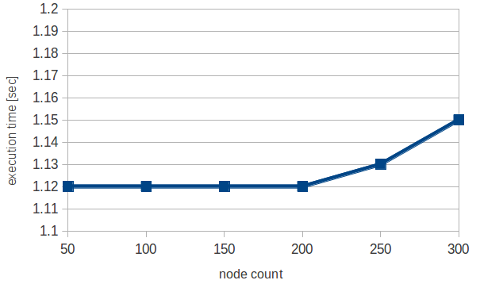
\includegraphics[width=\textwidth]{f2}
	\caption{}
	\label{fig:2}
\end{figure}

\begin{figure}
	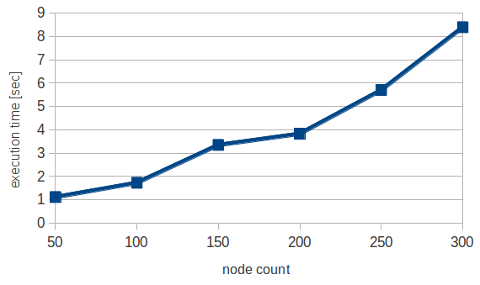
\includegraphics[width=\textwidth]{f3}
	\caption{}
	\label{fig:3}
\end{figure}

\section{Discussion}

We showed linear scalability of the dispatch – see Fig.~\ref{fig:1}, achieving below 10 sec (12 for Source catalog) times when run on the entire, 300 node cluster. Queries that touch all chunks on all clusters are required to complete under an hour, so 10-12 sec overhead is very low. During previous large scale tests we run on 150 nodes 2 years ago, we were getting $\sim$4 sec overhead. During this test, we measured 3.3 sec on 150-node configuration, which indicates we reduced the overhead, however since hardware used for these two tests was not the same, direct comparison would not be entirely fair.

We showed the overhead for simple, interactive queries was on the order of 1.8 sec when dispatching a query on one of the 300-nodes (Fig.~\ref{fig:2}). Yes, we can observe a non linearity starting from $\sim$200 nodes, however that non-linearity is on the order of 0.03 second when going from 200 to 300 nodes. Since we are required to answer interactive queries under 10 sec, the $<$20\% overhead is already acceptable, though we are planning to reduce it further in the future.

We were able to run all interactive-type queries well under required 10 second, with the exception of simple Object-Source join, which tool 11.2 sec. The longer-than-ideal time is attributed to unnecessary materialization of subchunks for every query that involves a join – this is expected to be optimized and alleviated in the near future.
More complex queries, such as a query that selects from a mid-size region showed linear scalability as well (Fig.~\ref{fig:3}). The one time 6-sec ``jump'' between 100 and 150 node test is attributed to switching to different number of chunks: as we reduced the size of the cluster from 150 to 100 nodes, we excluded some chunks that were previously falling inside searched region.

We were also able to run complex queries, such as full table scans and near neighbor queries, and did not observe any anomalies.

It is important to note that due to the ratio of data size to RAM, a large fraction of the data, in particular for the ``small'' Object catalog was cached in memory. Such environment was particularly good for testing dispatch and result returning overheads, however it would be unfair to approximate observed performance to production-size data sets, especially given that we also had a smaller number of chunks (3,000 in the test vs expected 20,000 in production).

\bibliography{lsst}

\end{document}
